\documentclass[conference]{IEEEtran}[10]
\IEEEoverridecommandlockouts
\usepackage{cite}
\usepackage{amsmath,amssymb,amsfonts}
\usepackage{graphicx}
\usepackage{textcomp}
\usepackage{xcolor}
\usepackage{float}
\usepackage{anyfontsize}
\usepackage {hyperref}
\usepackage{authblk}
\usepackage{caption}
\usepackage{subcaption}
\bibliographystyle{unsrtnat}
\begin{document}
\title{House Rent Prediction using polynomial and linear regression}
\author[1]{ Amit Roy
}
\affil[1]{ID: 2017-3-60-021
}

\author[2]{ Sirajum Maria Muna
}
\affil[2]{ID: 2017-3-60-020
}

\author[3]{ Shekhor Chandra Saha
}
\affil[3]{ID: 2017-3-60-025
}

\author[4]{ Saniat Injam
}
\affil[4]{ID: 2017-3-60-093
}

\maketitle
\IEEEpubidadjcol
\section{INTRODUCTION}
\subsection{1.1 Objectives}
With the mass growth of population around the world, it has become a challenge to provide accommodation for the people. As well as the growth of population the housing prices are also becoming high. For this reason, people opting for house renting as, owning a house seem like a dream like to some people. In this project our aim is to find house rent for a certain area in different cities. We are using a combination of linear regression and polynomial regression to predict house rent prices. 
\subsection{1.2 Motivation}
As we live in a third world country, also a over populated one, finding a good place to live a life peacefully is not easy. Along with ourselves, we want to secure a good future for our next generations. But money is always a problem. So, in this project we are motivated by this idea and tried to do a better approach, so that, it can help us by predicting the rental price to make us learn, on which area has better facilities in our suited budget. If anyone wants to further invest on real estates, this approach can help them. Also, it can be the parameter to signify one area’s demand.
\subsection*{1.3 Existing works}
Several machine learning algorithms have been used in the past years in this field. A study has been done in Fairfax County, Virginia using several machine learning algorithms like Naïve Bayes, Ripper, Decision Tree, Adaboost etc. to predict the house prices \cite{park2015using}.
Ridge and Lasso Linear regression is being used for house rent prediction \cite{kumar2019house}.
Also, Hybrid Linear Regression is being used by combining Ridge and Lasso along with Gradient Boosting combination to find more accurate predicted values with higher accuracy \cite{c3}.
By all these studies, what we have done till now, we have seen using hybrid machine learning algorithms gives better result than only one algorithm. Also, regression is a common classifier in that field. So, we have chosen to work on this part in our project.
\subsection*{1.4 Necessity}
As we have discussed in the motivation part, house rent prediction work can be used in daily basis to predict rental prices. In house rental dataset there can be several fractional values as well as non-numerical values. So, using regression is the safe option, as it works with fractional values and the non-numeric values can be pre-processed before the algorithm runs. Being less time consumption is another plus point of regression. The rental price prediction approach can ease many  manual work and gives people high efficient work facilities. 

\section{METHODOLOGY}
\begin{figure}[H]
\centering
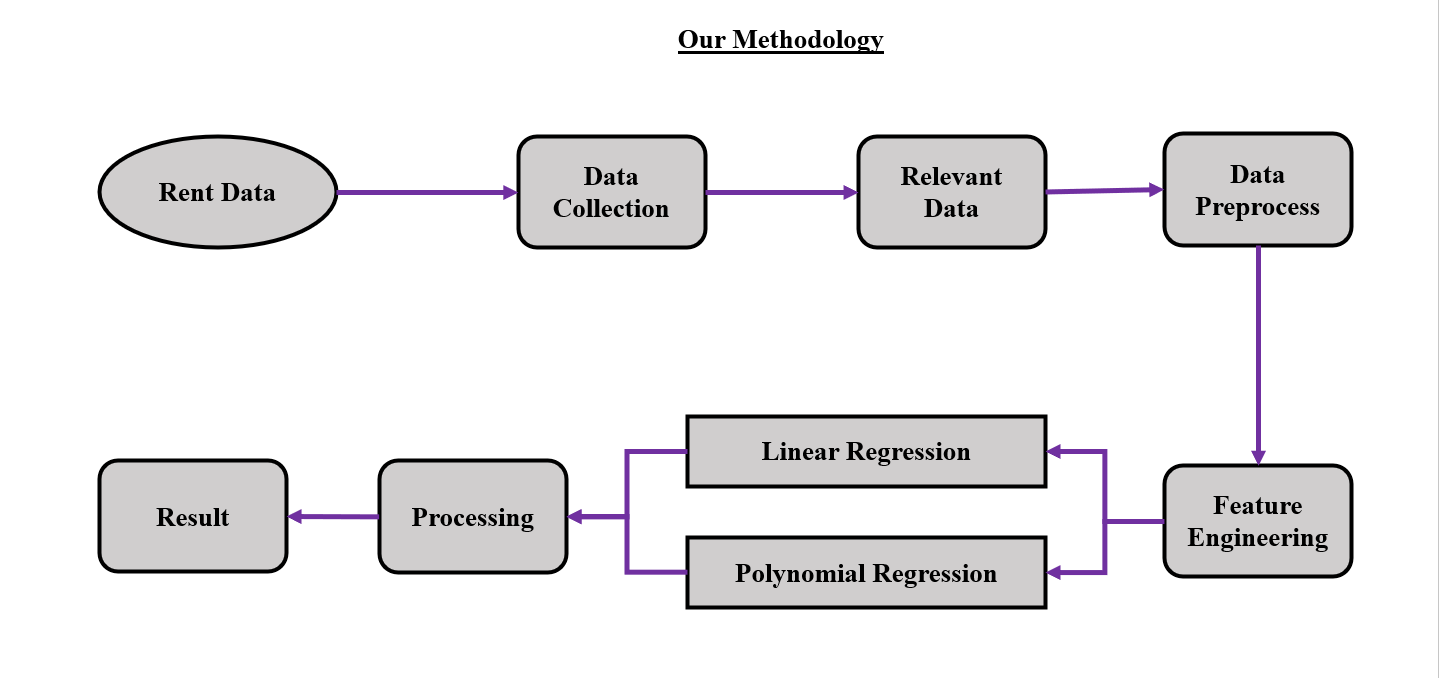
\includegraphics[scale=0.2]{methodology}
\caption{ Diagram of our proposed model}
\end{figure}
\section{IMPLEMENTATION}
\subsection{3.1 Data collection}
The data is collected from Kaggle. The dataset is based on the house rental prices of different cities in India. There are 1,93,011 rows and 10 columns. The price attribute is the dependent attribute where the other nine attributes (Seller-Type, Bedroom, Layout-Type, Property-Type, Area, Furnish-Type, Bathroom and City) are independent attributes. Seller-Type is divided into Owner, Agent and Builder. There are two types of Layout. BHK (Bedroom, Hall, Kitchen) and RK (Room and Kitchen). Property-Type has many sub-types, such as Apartment, Studio Apartment, Independent House, Villa, Independent Floor and Penthouse). Furnish-Type is divided into three types. Semi-Furnished, Un-Furnished and Furnished.  Cities are: Ahmedabad, Bangalore, Delhi, Chennai, Pune, Mumbai, Kolkata, Hyderabad. We can ensure that, all data in the dataset are authentic.
\subsection{3.2 Data processing}
Here we have dropped locality because, for each row we have different locality. And for all non-numerical data we have used one hot encoding to convert it into a numeric form.\\
For different types of property they assume them as different attributes. The encoding generates binary codes. A specific attribute has a specific binary number (0 or 1). 
\begin{figure}[H]
\centering
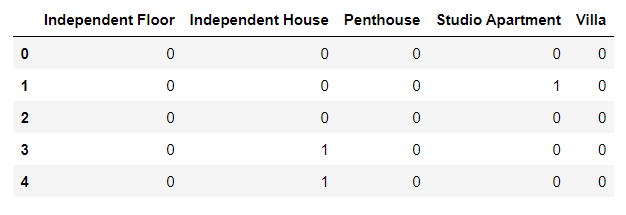
\includegraphics[scale=0.4]{one hot encoding}
\caption{ Non-numerical data processing by one hot encoding}
\end{figure}
For Seller-Type,Layout,Furnish-Type and City the non-numerical values are converted by same process.\\
After that, we have dropped the previous non-numeric attributes and store the dataset. Then, we have merged the encoded attributes with the stored dataset and will finally get a wholesome dataset ready for regression classification.
\subsection{3.3Model development}
We have worked with 2 types of regression: linear and polynomial regression and will estimate the accuracy between the models. In our final dataset we have 193011 rows and 21 columns. The dataset is divided according to the attributes in two sets: one is independent set, and another is dependent set. Then we have divided them by test (20\%) and train (80\%) data. In train set, there are 154408 data and in test set, we have 38603 data.

\textbf{Linear Regression(Simple and Multiple):}
Linear Regression is one of the well-known algorithms in machine learning. Basically, Linear Regression is used for predictive analysis. Linear regression is linear model that assumes a linear relationship between one or more independent variables and one dependent variable. There is a single input variable it is called simple linear regression. When there is more than one input variable it is called multiple linear regression.
\\\textbf{Equation of simple linear regression:}
\begin{center}
{\large Y = a + bX}
\end{center}
Where,
\\X is the explanatory variable,
\\Y is the dependent variable, 
\\B is the slope of the line,
\\a is the intercept (the value of y when x = 0).
\\\textbf{Equation of Multiple linear regression:}
\begin{center}
{\large yi = $\beta$0+$\beta$1xi1+$\beta$2xi2+...+$\beta$pxip+$\epsilon$}
\end{center}
where,
\\for i=n observations:
\\yi is the dependent variable,
\\xi is the explanatory variables,
\\$\beta$0 is the y-intercept (constant term),
\\$\beta$p  is the slope coefficients for each explanatory variable,
\\$\epsilon$ is the model’s error term (also known as the residuals).



\textbf{Polynomial Regression:}
Polynomial is one of the forms of regression analysis. Nonlinear relationship are fit by polynomial regression between the independent value and the corresponding conditional mean of dependent value. 
\\\textbf{Equation of Polynomial regression:}
\begin{figure}[H]
\centering

\includegraphics[scale=0.35]{pe}
\end{figure}
Where,
\\$\theta$0 is the bias,
\\$\theta$1, $\theta$2, …, $\theta$n are the weights in the equation of the polynomial regression,
\\and n is the degree of the polynomial.
\\The number of higher-order terms increases with the increasing value of n.
\subsection{3.4 Results}
We have run polynomial and linear regression function to train (80\%) our data. Then test these algorithms by 20\% train data. Based on the test data we have run three types of accuracy function. R2-score, MSE (Mean Square Error) and RMSE (root Mean Square Error) is being used to find which of these two regressions is best for the dataset.

\begin{figure}
     \centering
     \begin{subfigure}[b]{0.2\textwidth}
         \centering
         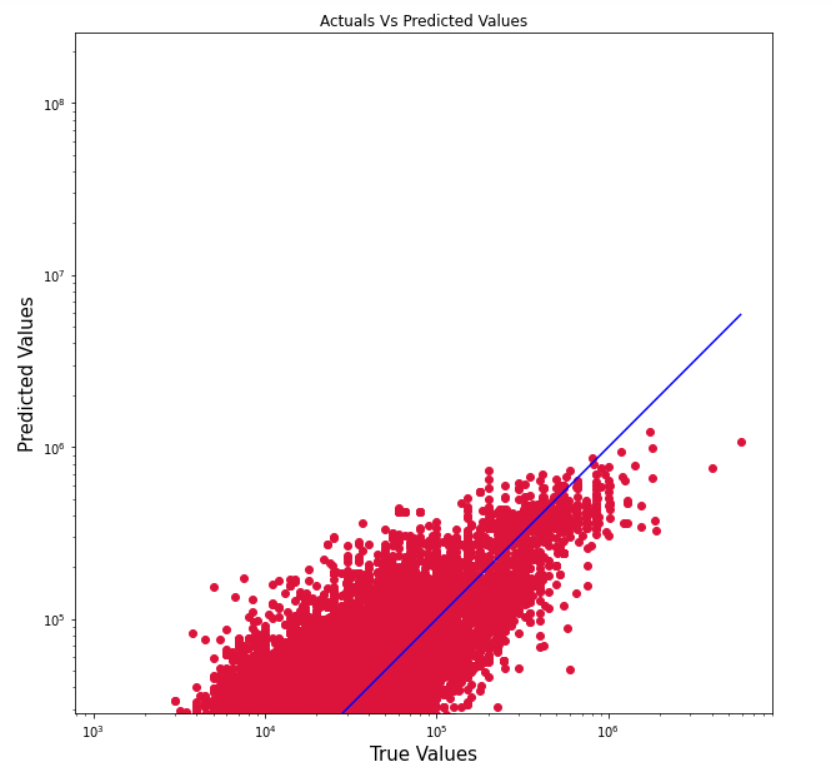
\includegraphics[width=\textwidth]{linear}
         \caption{Linear}
         \label{fig:Linear}
     \end{subfigure}
     \qquad
     \begin{subfigure}[b]{0.2\textwidth}
         \centering
         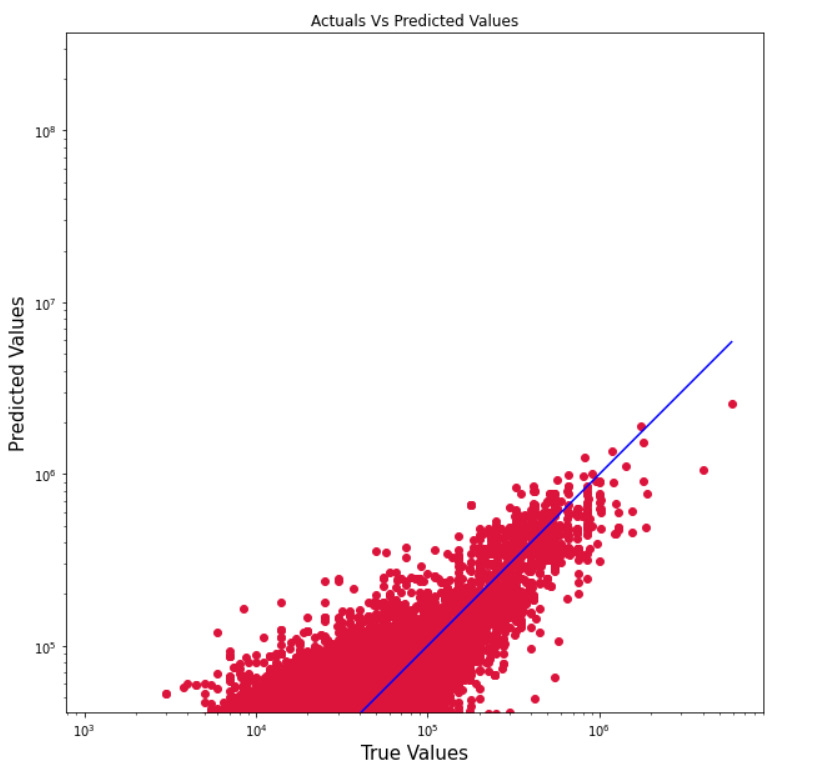
\includegraphics[width=\textwidth]{poly}
         \caption{Polynomial}
         \label{fig:Polynomial}
     \end{subfigure}
     
        \caption{Plot of linear and polynomial regression using expected and predicted values}
        \label{fig:Plot of linear and polynomial regression using expected and predicted values}
\end{figure}
Here, we can see that, in polynomial regression, the points are nearer to the best fitted line than the linear regression.

\begin{figure}[H]
\centering
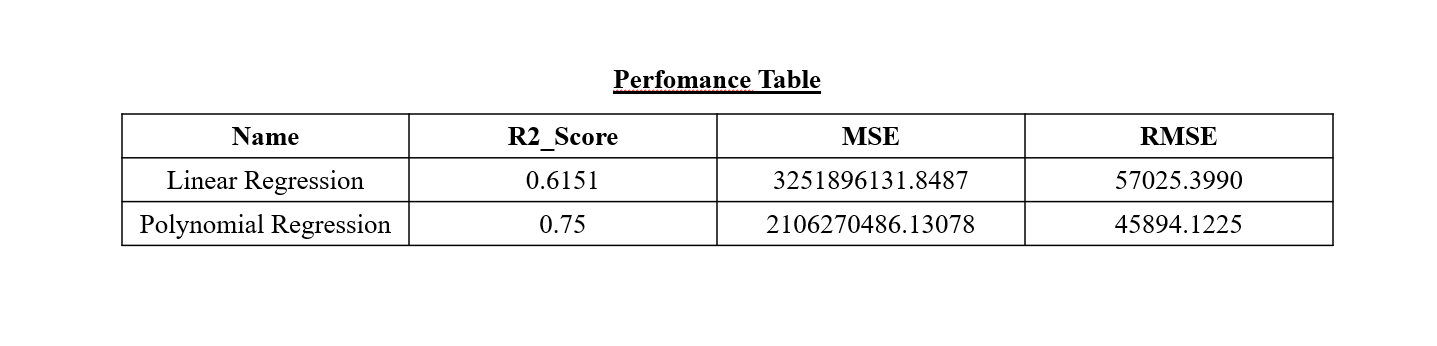
\includegraphics[scale=0.25]{performancetable}
\caption{ Accuracy table for linear and polynomial regression}
\end{figure}
\textbf{1.R2-Score:}
It is the statistical measurement, that shows how close is our data to the fitted line of the regression. The higher value of R2-Score represents the better fitted value of our data\cite{r2}. It provides the estimation of the strength relationship between response variable and our model.\\
\\
\textbf{R2-Score = SS\begin{footnotesize}
regression
\end{footnotesize}
/ SS\begin{footnotesize}
total
\end{footnotesize}
}\\
\\
Here, SS\begin{footnotesize}
regression
\end{footnotesize} means sum of squares. The square is between our predicted values and our test values and,\\
 SS\begin{footnotesize}
total
\end{footnotesize} means the total sum of squares which measures the variation of our observed data.\\
\\
\textbf{2.Mean Square Error:}
MSE is measured by calculating the distances(error) between the points to our regression line. In this case we need to calculate the average of the errors. The lowest MSE, the better model we get.In our observation, we get less MSE in polynomial regression.\\
\begin{figure}[H]
\centering
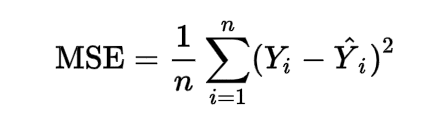
\includegraphics[scale=0.4]{mse}
\end{figure}
Here, n = number of data points\\
      Y\begin{footnotesize}
      i
      \end{footnotesize} = observed values and,\\
      $\widehat{Y}$\begin{footnotesize}
      i
      \end{footnotesize} = predicted values.\\
\\      
\textbf{3.Root Mean Square Error:}
It is the most commonly used accuracy model for linear regression. RMSE is the standard deviation of predicted errors.It also shows how concentrated the points are around the best fitted line.The root square of mean square error is the RMSE. Though RMSE is sometimes instinctive,in our model it works as it should be. 
\\
\section{CONCLUSIONS}
In this project our purpose was, to find and compare the accuracy between two types of linear regression models. for that, we have used linear regression and polynomial regression, and according to our test and trained data, the accuracy arrow shows that, in the renting price prediction model, if we use polynomial regression, we can get better result. We have used several accuracy model to prove our findings, as we have shown above.
\subsection{4.1 Challenges}
The main challenge for us, when we had started our project is to decide, which classification model should we use. We could not use decision tree because for each data tuple we can get different value. So it cannot be grouped easily. So, for being safe side and as we need to work with fractional values we have chosen regression model. To convert the non-numerical value was also a challenge for us. Though we have overcome it for our dataset.
\\
\subsection{4.2 Limitations}
In this project we have used dataset containing scattered values. If we show n the plots of Fig:3 and Fig:4 we can see that, most of the data is at a distance from the best fitted line. So, it could not give a better accuracy. If we can use a dataset containing data with less variation in one class, we hope it can give us better result.
\\
\subsection{4.3 Future directions}
We can flourish our model to a better version in the near future. Different kinds of evalution methods can be used. Using Cross validation method or Bootstrap can give it a better enlightenment according to our hypothesis. Though we have not tried that in our project, but we believe if we work on future we can make it to a better version and bring it to an another level.
\bibliographystyle{IEEEtran}
\bibliography{citation}
\medskip
\begin{thebibliography}{99}
\bibitem{r2} 
\texttt{https://corporatefinanceinstitute.com/
resources/knowledge/other/r-squared/\#tab=tab\_1}

\end{thebibliography}

\end{document}
